 \documentclass[12pt,a4paper]{article}
\usepackage{amsmath}
\usepackage{amssymb}
\usepackage{epstopdf}
\usepackage{inputenc}
\usepackage{graphicx}
\usepackage{titletoc} 
\usepackage{fancyhdr}   
\usepackage[a4paper,pdftex]{geometry}	
\usepackage[english]{babel}
\usepackage{xcolor} 
\usepackage{enumerate}
\usepackage{fix-cm} 
\usepackage[notlof]{tocbibind}
\usepackage{amsmath}
\usepackage{listings}
\usepackage{float}
\usepackage{enumitem}
\usepackage{xcolor}
\usepackage{listings}
\definecolor{vgreen}{RGB}{104,180,104}
\definecolor{vblue}{RGB}{49,49,255}
\definecolor{vorange}{RGB}{255,143,102}
\renewcommand\lstlistingname{Appendix}
\renewcommand\lstlistlistingname{Appendix}

\lstdefinestyle{verilog-style}
{
	language=Verilog,
	basicstyle=\small\ttfamily,
	keywordstyle=\color{vblue},
	identifierstyle=\color{black},
	commentstyle=\color{vgreen},
	moredelim=*[s][\colorIndex]{[}{]},
	frame=single,
	literate=*{:}{:}1
}

\makeatletter
\newcommand*\@lbracket{[}
\newcommand*\@rbracket{]}
\newcommand*\@colon{:}
\newcommand*\colorIndex{%
	\edef\@temp{\the\lst@token}%
	\ifx\@temp\@lbracket \color{black}%
	\else\ifx\@temp\@rbracket \color{black}%
	\else\ifx\@temp\@colon \color{black}%
	\else \color{vorange}%
	\fi\fi\fi
}
\makeatother

\usepackage{trace}

\usepackage{subcaption}
\begin{document}
	\begin{titlepage}
		\begin{center}
			
\includegraphics[scale=1.5]{figures/CoverSheet}\\
			\bf{ \small{DEPARTMENT OF ELECTRICAL AND ELECTRONIC ENGINEERING} }
		\end{center}
		
		\vspace{4cm}
		\centering
		\textbf{\Huge Assignment 2}
		
		\vspace{1cm}
		
		{\Large MIPS Single-cycle Processor}
		
		\vspace{4cm}
		
		\textbf{\LARGE Sahand Sabour}
		
		\vspace{2cm}
		
		\textbf{\large EEE339}
		
		\vspace{0.5cm}
		
		{\large Digital System Design with HDL(II)}
		
		\vspace{1.5cm}
		
		\textbf{\large Student ID}
		
		\vspace{0.5cm}
		
		{\large 1614650}
		
		\vfill
		
	\end{titlepage}

	\noindent \textbf{\Large Introduction}
	\vspace{0.2cm}
	
	\noindent With the significant growth of computers and electronic devices, mastering computer architecture has become highly essential for the engineers of this field. Computer architecture can be mainly divided to two fields: Instruction set design and design of machine hardware organization. The EEE339 course focuses on the prior field. The instruction set is a group of instructions that are written in binary, that are designed to carry out a series of operations. The instruction set used for this assignment is MIPS, which is originally developed by MIPS Technologies.  
	
	\noindent In this assignment, a MIPS single-cycle processor is implemented using Verilog. Moreover, several instruction sets are designed to conduct the instructed tasks. The machine code corresponding to each task, the obtained simulation results, and thorough explanation of the design process is provided in this report. In addition, required changes to the processor design are demonstrated in the relative sections.
	
	\vspace{0.5cm}
	\noindent \textbf{\large Task 1}
	\vspace{0.2cm}
	
	\noindent \textbf{ a)} The following machine code loads the data stored in memory X to the X register, where X is 1.
	
	\begin{table}[H]
		\centering
		\begin{tabular}{|c | c| c| c|}
			\hline
			\textbf{Opcode} & \textbf{rs} & \textbf{rt}& \textbf{offset address}\\ \hline
			100011& 00000 & 00001 & 0000000000000001\\\hline
		\end{tabular}
	\end{table}

	\noindent Moreover, the following machine code would load the data stored in memory Y to Y register, with Y being 2.
	\begin{table}[H]
		\centering
		\begin{tabular}{|c | c| c| c|}
			\hline
			\textbf{Opcode} & \textbf{rs} & \textbf{rt}& \textbf{offset address}\\ \hline
			100011& 00000 & 00010 & 0000000000000010\\\hline
		\end{tabular}
	\end{table}

	\noindent In the above code, 100011 for opcode corresponds to the load word (lw) instruction. The addition of the rs and offset address fields corresponds to the memory location while the rt field determines the register number to load the data into. Hence, the above values were decided.
	
	\vspace{0.4cm}
	\noindent \textbf{ b)}  In order to add the values of X and Y registers and store the obtained value in the Z register, the adding operation is to be used, which is an R-type instruction. Hence, the opcode should be set to 000000. Accordingly, the values of rs and rt should be set to the address of registers X and Y respectively, which would be 00001 and 00010. The register number for the Z register would be set in the rd field. Hence, this field should be set to 00011 as the the value of Z is instructed to be 2. As there is no shift required for this operation, the value of shamt is set to 00000. Conclusively, the value of the funct field would be set to the machine code for the addition operation, which is 100000. 
	The following machine code would be obtained as the result.
	
	\begin{table}[H]
		\centering
		\begin{tabular}{|c | c| c| c|c|c|}
			\hline
			\textbf{Opcode} & \textbf{rs} & \textbf{rt} & \textbf{rd}& \textbf{shamt}& \textbf{funct}\\ \hline
			000000& 00001 & 00010 &00011&00000&100000 \\\hline
		\end{tabular}
	\end{table}

	\vspace{0.4cm}
	\noindent \textbf{ c)} The following machine code is used to store the data from Z register into Z memory location.
	
	\begin{table}[H]
		\centering
		\begin{tabular}{|c | c| c| c|}
			\hline
			\textbf{Opcode} & \textbf{rs} & \textbf{rt}& \textbf{offset address}\\ \hline
			101011& 00000 & 00011 & 0000000000000011\\\hline
		\end{tabular}
	\end{table}
	
	\noindent The opcode 101011 corresponds to the instruction code for the store word (Sw) instruction. The addition of the rs and offset address fields would determine the memory location to store the data into, while rt represents the register to obtain the data from. Hence, the above values were decided. 
	
	\vspace{0.4cm}
	\noindent \textbf{ d)} Loading the data from the Z memory location into the T register uses the same operation as section a: using the loadword operation. In this case, the addition of the rs and offset address fields should correspond to the Z memory location while the rt field corresponds to the T register, which is instructed to be 3. Hence, the following machine code was decided. 
	
	\begin{table}[H]
		\centering
		\begin{tabular}{|c | c| c| c|}
			\hline
			\textbf{Opcode} & \textbf{rs} & \textbf{rt}& \textbf{offset address}\\ \hline
			100011& 00000 & 00100 & 0000000000000011\\\hline
		\end{tabular}
	\end{table}

	\noindent The full machine code for task 1 is provided in the figure below (Figure 1).
	
	\begin{figure}[H]
		\centering
		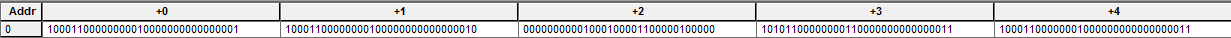
\includegraphics[height=1cm,width=14cm]{figures/code1.png}
		\caption{The instruction set for task 1}
	\end{figure}
	
	\vspace{0.2cm}
	\noindent \textbf{\large Task 2}
	\vspace{0.2cm}
	
	\noindent In order to display the content of X, Y, and T registers, as well as the PC, several modifications should be made to the design of the processor as these values are not declared as outputs in the original design. Hence, the modules are to be analyzed from bottom to top level.
	
	\noindent The RegisterFile module contains the registers' data and operations. However, this module only outputs the register values read. Therefore, the X, Y, and T registers should also be declared as outputs. Accordingly, the modified module would be as follows: 
	\begin{lstlisting}[style={verilog-style}]
module RegisterFile (Read1,Read2,Writereg,WriteData,RegWrite, 
Data1, Data2,clock,reset, X, Y, T); // added to parameters

input 	[4:0] Read1,Read2,Writereg;
input 	[31:0] WriteData;// data to write
input 	RegWrite;// The write control
input 	clock, reset;// The clock to trigger writes
output 	[31:0] Data1, Data2;// the register values read;
output reg [31:0] X, Y, T; // for simulation purposes
reg 	[31:0] RF[31:0];// 32 registers each 32 bits long
integer	k;

// Read from registers independent of clock	
assign 	Data1 = RF[Read1];
assign 	Data2 = RF[Read2]; 
// write the register with new value on the falling edge of 
// the clock if RegWrite is high
always @(posedge clock or posedge reset)
begin
if (reset) for(k=0;k<32;k=k+1) RF[k]<=32'h00000000;
// Register 0 is a read only register with the content of 0
else if (RegWrite & (Writereg!=0)) RF[Writereg] <= WriteData;
// Writing the values of first, second, and forth registers
// to the correponding variables
// The table instructs X, Y, and T to be 1,2,4 respectively
begin 
	X<= RF[1];
	Y<= RF[2];
	T<= RF[4];
end
end
endmodule
	\end{lstlisting}
	 
	 \noindent An instance of this module is created in the DataPath module. Hence, the parameters for this instance should be updated as follows. 
	
	\begin{lstlisting}[style={verilog-style}]
// Instantiate Register File (updated)
RegisterFile REG(rs, rt, WriteReg, RWriteData, RegWrite, 
ALUAin, DWriteData,clock,reset, X, Y, T);
	\end{lstlisting}
	
	\noindent Accordingly, the mentioned registers must be declared as outputs. In addition, as the PC should also be shown in the simulations, it would be added to the list of outputs likewise (see below code).
	
	\vspace{-0.3cm}
	\begin{lstlisting}[style={verilog-style}]
output	[31:0]	X, Y, T, PC;
	\end{lstlisting}
	
	\noindent Similar to the modifications in the previous module, the declared outputs must be added to the module parameters as below.
	
	\vspace{-0.3cm}
	\begin{lstlisting}[style={verilog-style}]
// Datapath
module DataPath(RegDst, Branch, MemRead, MemtoReg, ALUOp, 
MemWrite,ALUSrc, RegWrite, clock, reset, opcode,ALUResultOut,
DReadData, X, Y, T, PC);
	\end{lstlisting}
	
	\noindent Lastly, the top-level is to be updated likewise. In the MIPS1CYCLE module, an instance of the DataPath module is created. Hence, the parameters for this instance should be updated. 

	\vspace{-0.3cm}
	\begin{lstlisting}[style={verilog-style}]
// Instantiate the Datapath (updated)
DataPath MIPSDP (RegDst,Branch,MemRead,MemtoReg,ALUOp,
MemWrite,ALUSrc,RegWrite,clock, reset, opcode, ALUResultOut,
DReadData, X, Y, T, PC);
	\end{lstlisting}
	
	\noindent Correspondingly, the registers and the PC should be declared as outputs, similar to the modifications in the previous modules. 
	
		\vspace{-0.4cm}
	\begin{lstlisting}[style={verilog-style}]
output	[31:0]	X, Y, T, PC;
	\end{lstlisting}
	
	\noindent The parameters for this module are to be updated as below likewise. 
	
		\vspace{-0.4cm}
\begin{lstlisting}[style={verilog-style}]
module MIPS1CYCLE(clock, reset,opcode, ALUResultOut,
DReadData, X, Y, T, PC);
\end{lstlisting}
	
	\noindent The simulation result of running the program in task 1 is displayed in the below figure (Figure 2). 
	
	\begin{figure}[H]
		\centering
		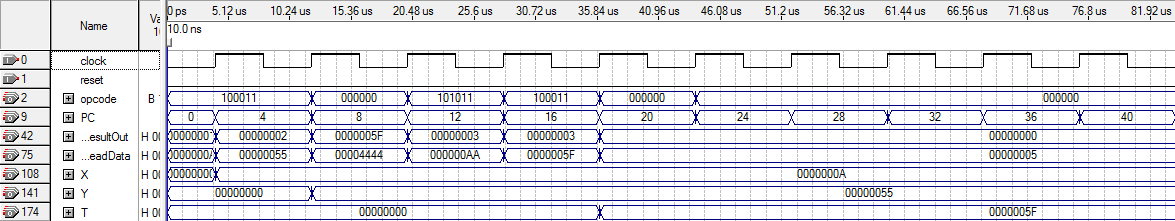
\includegraphics[height=4.1cm,width=15cm]{figures/simulations1.png}
		\caption{Task 1 results}
	\end{figure}
	
	\noindent As illustrated in the figure, the values from the designated memory locations are loaded into corresponding registers; that is, the value 0000000A is loaded from memory 1 to register 1 (X), the value 00000055 is loaded from memory 2 to register 2 (Y), and the addition results of the two registers, which is equal to 0000005F, is stored in register 4 (T). ALUResultOut displays the calculated memory location for Load/Store instructions and shows the calculation results for R-type instructions. Evidently, the obtained results show that the operation has been implemented correctly.

	\vspace{0.4cm}
	\noindent \textbf{\large Task 3}
	\vspace{0.2cm}
	
	\noindent In order to simulate the BEQ operation, two sets of instructions were designed: First, equal values are processed to show that the branching operation is functional. Second, non-equal values are processed to demonstrate that the branching function would not be called if the equivalence condition is not met. 
	
	\noindent Initially, the values from data memories X and Y would be loaded to the corresponding registers respectively. The same instruction code as task 1 is used to achieve this operation. 
	
	\noindent The opcode for the BEQ operation is 000100. The rs and rt fields correspond to the registers whose values are to be compared. The offset address determines the change in the PC value divided by 4. Hence, setting the offset value to 1 would skip the instruction after the BEQ instruction.
	
	\begin{table}[H]
		\centering
		\begin{tabular}{|c | c| c| c|}
			\hline
			\textbf{Opcode} & \textbf{rs} & \textbf{rt}& \textbf{offset address}\\ \hline
			000100& 00001 & 00001 & 0000000000000001\\\hline
		\end{tabular}
	\end{table}
	
	\noindent In the above machine code, the same register is used for rs and rt fields in order to trigger the branch operation. Accordingly, two arbitrary instructions to follow the BEQ instruction were decided. The result of these instructions were believed to better demonstrate the BEQ operation. The first instruction would load the value from memory Y to register X and the second instruction would load the value of memory X to register T. The machine code for these two instructions is provided below respectively.
	
	\begin{table}[H]
		\centering
		\begin{tabular}{|c | c| c| c|}
			\hline
			\textbf{Opcode} & \textbf{rs} & \textbf{rt}& \textbf{offset address}\\ \hline
			100011& 00000 & 00001 & 0000000000000010\\\hline
		\end{tabular}
	\end{table}

\vspace{-0.5cm}

	\begin{table}[H]
		\centering
		\begin{tabular}{|c | c| c| c|}
			\hline
			\textbf{Opcode} & \textbf{rs} & \textbf{rt}& \textbf{offset address}\\ \hline
			100011& 00000 & 00100 & 0000000000000001\\\hline
		\end{tabular}
	\end{table}
	 
	\noindent The complete instruction set for this step is provided in Figure 3.
	
	\begin{figure}[H]
		\centering
		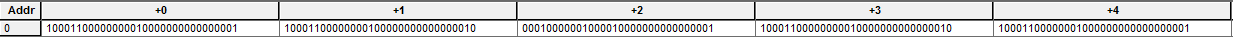
\includegraphics[height=1cm,width=14cm]{figures/code2.png}
		\caption{The instruction set for first step of task 3}
	\end{figure}

	\noindent The simulation result for this step is displayed in the figure below (Figure 4). As shown in the figure, the value of pc is incremented by 8 rather than 4 as the branching condition has been met. Moreover, it can be seen that the value from memory Y is not loaded to register X. Hence, this instruction is skipped.
	
	\begin{figure}[H]
		\centering
		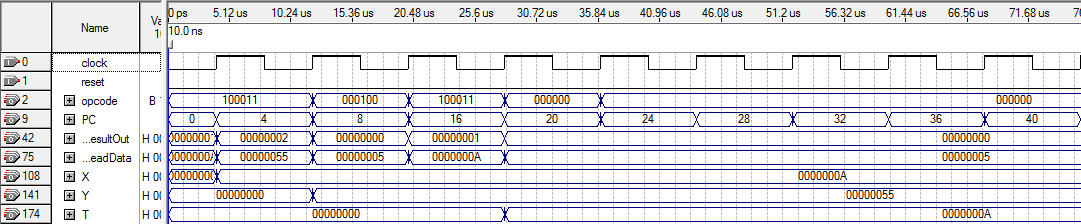
\includegraphics[height=5cm,width=15cm]{figures/simulations2.png}
		\caption{Task 3 results - step 1}
	\end{figure}

	\noindent In the second step, two registers with different values would be compared (arbitrarily values of X and Y registers). The machine code for this instruction is as below. 
	
	\begin{table}[H]
		\centering
		\begin{tabular}{|c | c| c| c|}
			\hline
			\textbf{Opcode} & \textbf{rs} & \textbf{rt}& \textbf{offset address}\\ \hline
			000100& 00001 & 00010 & 0000000000000001\\\hline
		\end{tabular}
	\end{table}

	\noindent The full instruction set for this step is provided in Figure 5.
	
	\begin{figure}[H]
		\centering
		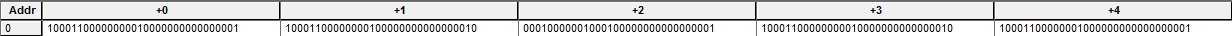
\includegraphics[height=1cm,width=14cm]{figures/code3.png}
		\caption{The instruction set for first step of task 3}
	\end{figure}

	\noindent The simulation result for this step is illustrated in Figure 6. As shown in the figure, the PC value is constantly incremented by 4. Moreover, it can be seen that in addition to the loading of value from memory X to register T, the value from memory Y is loaded to register X likewise. Hence, the branching operation was not called due to the values being not equal.
	
	\begin{figure}[H]
		\centering
		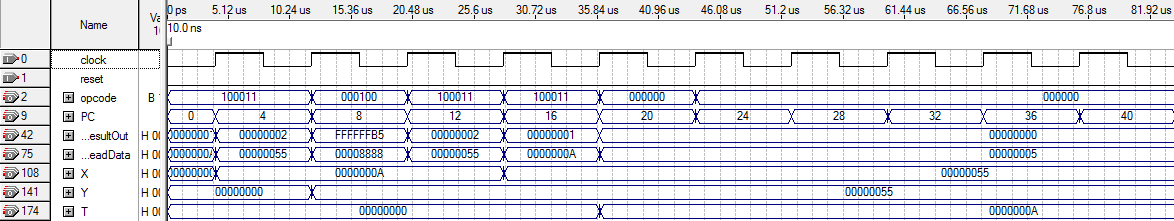
\includegraphics[height=4.1cm,width=15cm]{figures/simulations3.png}
		\caption{Task 3 results - step 2}
	\end{figure}

	\vspace{-0.2cm}
	\noindent Conclusively, the BEQ instruction was implemented successfully.

	\vspace{0.4cm}
	\noindent \textbf{\large Task 4}
	\vspace{0.2cm}
	
	\noindent The Jump instruction consists of a 6-bit opcode and a 26-bit address, which is the address of the instruction to jump to. In order to implement this instruction, its design is to be added to the Control module. The opcode for the Jump instruction was chosen to be 000010. Moreover, as this instruction does not include any arithmetic operations and would only need a branch operation, the value of Branch and ALUOP would be set to 1 and 11 respectively while the other signals are set to either 0 or don't cares, similar to the BEQ instruction; the value of ALUOP is set to 11 as there is no corresponding ALU operation for this value. The updated Control module would be as below. 
	
	\vspace{-0.4cm}
	\begin{lstlisting}[style={verilog-style}]
// Main Controller
module Control (opcode,RegDst,Branch,MemRead,MemtoReg,
ALUOp,MemWrite,ALUSrc,RegWrite);

input 	[5:0] 	opcode;
output	[1:0] 	ALUOp;
output	RegDst,Branch,MemRead,MemtoReg,MemWrite,ALUSrc,
RegWrite;
reg	[1:0]	ALUOp;
reg 	RegDst,Branch,MemRead,MemtoReg,MemWrite,ALUSrc,
RegWrite;

parameter R_Format = 6'b000000, LW = 6'b100011, 
SW = 6'b101011, BEQ=6'b000100, JMP=6'b000010;
always @(opcode)begin
case(opcode)
R_Format:{RegDst,ALUSrc,MemtoReg,RegWrite,MemRead,MemWrite,
Branch,ALUOp}= 9'b 100100010;
LW: {RegDst,ALUSrc,MemtoReg,RegWrite,MemRead,MemWrite,
Branch,ALUOp}= 9'b 011110000; 
SW: {RegDst,ALUSrc,MemtoReg,RegWrite,MemRead,MemWrite,
Branch,ALUOp}= 9'b x1x001000;	
BEQ:{RegDst,ALUSrc,MemtoReg,RegWrite,MemRead,MemWrite,
Branch,ALUOp}= 9'b x0x000101; 
// added instructions
JMP:{RegDst,ALUSrc,MemtoReg,RegWrite,MemRead,MemWrite,
Branch,ALUOp}= 9'b x0x000111;

default: {RegDst,ALUSrc,MemtoReg,RegWrite,MemRead,MemWrite,
Branch,ALUOp}= 9'b xxxxxxxxx;
endcase
end
endmodule 
	\end{lstlisting}
	
	\noindent As mentioned previously, unlike the BEQ instruction, the Jump instruction does not determine the PC offset but rather determines the PC address itself. Hence, the PC value to be used for this instruction has to updated correspondingly in the DataPath module.
	
	\begin{lstlisting}[style={verilog-style}]
assign	PCValue	= (Branch & Zero)? (opcode == 6'b000010 ? 
SignExtendOffset:PC+4+PCOffset) : PC+4;
\end{lstlisting}
	
	\noindent The above addition to the design would set the PC value as the address for the Jump instruction and as the sum of the current value with the given offset for the BEQ instruction.
	
	\noindent In order to simulate the Jump instruction, two arbitrary instructions were used in prior: the instructions to load the data from memories X and Y to corresponding registers, similar to task 1. Consequently, the Jump instruction was used to branch back to the first instruction, thus making an infinite loop. Therefore, the machine code for this instruction would be as follows. 
	
	\begin{table}[H]
		\centering
		\begin{tabular}{|c | c|}
			\hline
			\textbf{Opcode}& \textbf{Address}\\ \hline
			000010 & 0000000000000000\\\hline
		\end{tabular}
	\end{table}

	\noindent The complete instruction set for this task is provided in Figure 7.
	
	\begin{figure}[H]
		\centering
		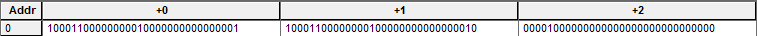
\includegraphics[height=1cm,width=14cm]{figures/code4.png}
		\caption{The instruction set for task 4}
	\end{figure}
	
	\noindent The obtained results from the simulation of the above instruction set is provided in the figure below (Figure 8).
	
	\begin{figure}[H]
		\centering
		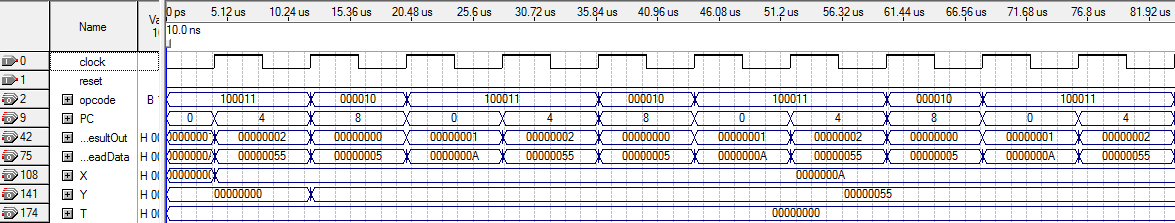
\includegraphics[height=4.1cm,width=15cm]{figures/simulations4.png}
		\caption{Task 4 results}
	\end{figure}

	\noindent As illustrated by the figure, the pc value is constantly reset to 0 when the Jump instruction is reached. Hence, it can concluded that the Jump instruction was successfully implemented.
	
	\vspace{0.4cm}
	\noindent \textbf{\large Task 5}
	\vspace{0.2cm}
	
	\noindent In order to add the additional instruction ORI, several modules were to be modified. Similar to the previous task, changes to the Control module had to be made in order to add a new instruction. The opcode for this instruction was decided to be 000001. The modified section of this module is provided below.
	
	\begin{lstlisting}[style={verilog-style}]
parameter R_Format = 6'b000000, LW = 6'b100011, 
SW = 6'b101011, BEQ=6'b000100, JMP=6'b000010;
always @(opcode)begin
case(opcode)
// added instructions
JMP:{RegDst,ALUSrc,MemtoReg,RegWrite,MemRead,MemWrite,
Branch,ALUOp}= 9'b x0x000111;

ORI:{RegDst,ALUSrc,MemtoReg,RegWrite,MemRead,MemWrite,
Branch,ALUOp}= 9'b 010100011;

default: {RegDst,ALUSrc,MemtoReg,RegWrite,MemRead,MemWrite,
Branch,ALUOp}= 9'b xxxxxxxxx;
\end{lstlisting}
	
	\noindent For this instruction, ALUSrc signal should be set to high as the second operand comes from the sign extended, lower 16-bits of the instruction. RegWrite signal was set to high likewise as the register on the write register input is expected to be written by the value on the write data input. Additionally, the ALUOp signal was set to 11. Hence, modifications to the ALUControl module were required, as ALUOp = 2'b11 would now correspond to both Jump and ORI instructions. 
	
	\vspace{0.1cm}
	\noindent In order to distinguish between the Jump and the ORI instructions, it was decided that the opcode would be sent to the ALUControl module as one of its inputs. Consequently, the arithmetic operation could be chosen based on the instruction. The mentioned modifications are provided below.
	
	\begin{lstlisting}[style={verilog-style}]
//ALU Control 
module ALUControl (ALUOp, FuncCode, ALUCtl, opCode);

	input 	[1:0] 	ALUOp;
	input 	[5:0] 	FuncCode;
	input 	[5:0] 	opCode; // declare as input
	output	[3:0]	ALUCtl;
	reg	[3:0]	ALUCtl;
	
	always@( ALUOp, FuncCode)
	begin
	case(ALUOp)
	2'b00:	ALUCtl = 4'b0010;
	2'b01:	ALUCtl = 4'b0110;
	2'b10:	case(FuncCode)
		6'b 100000: ALUCtl = 4'b 0010;
		6'b 100010: ALUCtl = 4'b 0110;
		6'b 100100: ALUCtl = 4'b 0000;
		6'b 100101: ALUCtl = 4'b 0001;
		6'b 101010: ALUCtl = 4'b 0111;
		default:	ALUCtl = 4'b xxxx;
		endcase
	2'b11: ALUCtl=(opCode== 6'b000010)?4'bxxxx:4'b0001;
	default:ALUCtl = 4'b xxxx;
	endcase
	end
endmodule
	\end{lstlisting}
	
	\noindent Where 0001 is the function code for OR operation. Accordingly, the created instance of this module in the DataPath has to be updated.
	
		\begin{lstlisting}[style={verilog-style}]
//Instantiate local ALU controller
ALUControl alucontroller(ALUOp,funct,ALUctl, opCode);
	\end{lstlisting}
	
	\vspace{0.4cm}
	\noindent \textbf{\large Task 6}
	\vspace{0.2cm}
	
	\noindent In order to simulate the results for the ORI operation, the instruction set was decided to include two instructions: first, load the data from memory X to register X, similar to task 1. Second, apply the ORI instruction between the data in register X and an arbitrary value, and store the results in register X. The machine code for the ORI instruction is as below. 
	\begin{table}[H]
		\centering
		\begin{tabular}{|c | c| c| c|}
			\hline
			\textbf{Opcode} & \textbf{rs} & \textbf{rt}& \textbf{offset address}\\ \hline
			000001& 00001 & 00001 & 0000000000000111\\\hline
		\end{tabular}
	\end{table}

	\noindent The complete instruction set for this task is displayed in Figure 9.
	
	\begin{figure}[H]
		\centering
		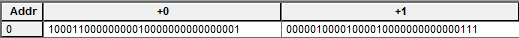
\includegraphics[height=1cm,width=14cm]{figures/code5.png}
		\caption{The instruction set for task 6}
	\end{figure}

	\noindent Moreover, the simulation results from running the above machine codes is displayed in the below figure (Figure 10).
	
		
	\begin{figure}[H]
		\centering
		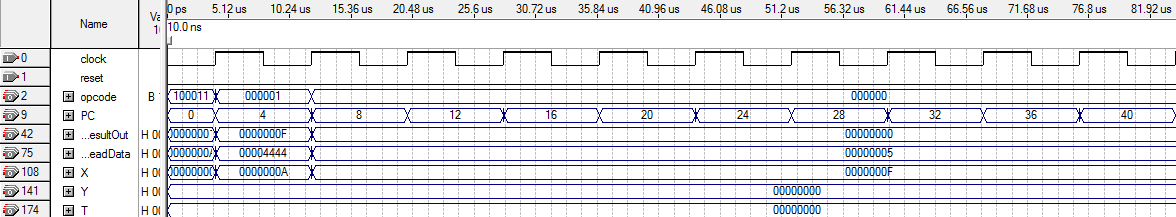
\includegraphics[height=5cm,width=15cm]{figures/simulations5.png}
		\caption{Task 6 results}
	\end{figure}

	\noindent According to the above figure, the data from memory X, which is 00000000A in hex (00000000000000000000000000001010 in binary), is loaded to register X. Consequently, the ORI instruction is used to apply the OR operation between this value and an arbitrary binary value 0000000000000111. Evidently, the result of this operation would be 00000000000000000000000000001111 in binary, which is 00000000F in hex. Hence, the ORI operation is functional and was implemented successfully. 
	
	\newpage
	\noindent \textbf{\large Task 7}
	\vspace{0.2cm}
	
	\noindent In order to change the the bus width from 32 to 20 (as indicated in the table), variable declarations were to be changed in several modules. More specifically, the variables relating to the data bus would be modified to be 20 bits rather than 32 bits. The mentioned changes for each module that required modifications is provided below respectively.
	
		\vspace{-0.4cm}
	\begin{lstlisting}[style={verilog-style}]
// Changes in the RegisterFile module
input 	[19:0] WriteData; // data to write
output 	[19:0] Data1, Data2; // the register values read;
output reg [19:0] X, Y, T;
reg 	[19:0] RF[31:0]; // 32 registers each 20 bits long
integer	k;
	
// The reset value for each register also has to be 20 bits
if (reset) for(k=0;k<32;k=k+1) RF[k]<=20'h00000000;
	\end{lstlisting}
	
		\vspace{-0.4cm}
	
	\begin{lstlisting}[style={verilog-style}]
// Changes in the MIPSALU module
input	[19:0] 	A,B;
output	[19:0] 	ALUOut;
reg	[19:0] ALUOut;
\end{lstlisting}
	\vspace{-0.4cm}

	\begin{lstlisting}[style={verilog-style}]
// Changes in the DataMemory module
input 	[19:0] 	Address, DWriteData;
output 	[19:0]	DReadData;
\end{lstlisting}
	\vspace{-0.4cm}

	\begin{lstlisting}[style={verilog-style}]
// Changes in the DataPath module
output	[19:0]	X, Y, T, ALUResultOut ,DReadData, PC;
wire  [19:0] 	SignExtendOffset,DWriteData,RWriteData, 
DReadData, ALUAin, ALUBin,DAddress, DmemOut,ALUResultOut;
\end{lstlisting}
	\vspace{-0.4cm}

	\begin{lstlisting}[style={verilog-style}]
// Changes in the MIPS1Cycle module
output	[19:0]	ALUResultOut ,DReadData, X, Y, T; 
wire [19:0] SignExtend,ALUResultOut ,DReadData;
\end{lstlisting}

	\vspace{0.4cm}
\noindent As displayed in the below figure (Figure 11), the same instruction set as task 1 is used. 

\begin{figure}[H]
	\centering
	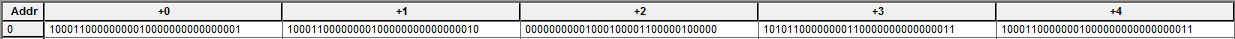
\includegraphics[height=1cm,width=14cm]{figures/code6.png}
	\caption{The instruction set for task 7}
\end{figure}

	\noindent Correspondingly, the simulation results for this task are provided in Figure 12. As illustrated by the figure, the data from memories X and Y has been loaded to their corresponding registers, and the addition result from memory z has been loaded to register T accordingly. The mere difference to be seen between the results of this section and task 2 would be data bus width, that is changed from 32 bits (8 bits in hex) to 20 bits (5 bits in hex).
		
	\begin{figure}[H]
		\centering
		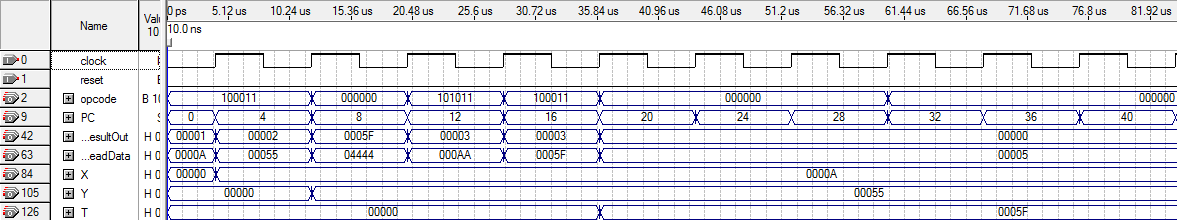
\includegraphics[height=5cm,width=15cm]{figures/simulations6.png}
		\caption{Task 7 results}
	\end{figure}

\vspace{-0.4cm}
	\noindent Based on the obtained results, it can be concluded that the bus width modification has been applied successfully. 

\vspace{0.4cm}
	\noindent \textbf{\Large Conclusion}
	\vspace{0.2cm}
	
	\noindent In conclusion, the design of a MIPS single-cycle processor was analyzed and modified to complete a series of given tasks. Thorough explanation of the decided instruction sets as well as the corresponding simulation results and the required modifications to the processor's design were provided. Based on the obtained results, it is believed that each of the given tasks were performed successfully. It is believed that this assignment was a valuable experience to learn more about the MIPS computer architecture design as well an assessment of the student's knowledge on the subject. 
	

\end{document}